\documentclass[aspectratio=169,10pt]{beamer}
\usetheme{Madrid}
\usecolortheme{seahorse}

\usepackage{amsmath}
\usepackage{amssymb}
\usepackage{amsfonts}
\usepackage{graphicx}
\usepackage{listings}
\usepackage{xcolor}
\usepackage{tikz}
\usepackage{multirow}

% Configure listings for code
\lstset{
    basicstyle=\ttfamily\scriptsize,
    commentstyle=\color{green!50!black}\itshape,
    keywordstyle=\color{blue}\bfseries,
    stringstyle=\color{red},
    numbers=left,
    numberstyle=\tiny\color{gray},
    breaklines=true,
    breakatwhitespace=true,
    frame=single,
    language=Python,
    showstringspaces=false,
    tabsize=2
}

% Set graphics path
\graphicspath{{figures/}}

% Title and author
\title{Chapter 8b: Integral Equations and Computational Schemes}
\subtitle{Applications of Monotone Operator Theory}
\author{Pathak, R. P.}
\date{An Introduction to Nonlinear Analysis and Fixed Point Theory}

\setbeamertemplate{footline}[frame number]

\begin{document}

% Title slide
\begin{frame}
    \titlepage
\end{frame}

% Table of contents
\begin{frame}{Outline}
    \tableofcontents
\end{frame}

% ============================================================================
\section{Introduction: Integral Equations}
% ============================================================================

\begin{frame}{Integral Equations in Applied Mathematics}
    \begin{itemize}
        \item Many physical phenomena modeled by integral equations
        \vspace{0.3cm}
        \item Classical types:
            \begin{itemize}
                \item Fredholm equations
                \item Volterra equations
                \item Hammerstein equations
                \item Urysohn equations
            \end{itemize}
        \vspace{0.3cm}
        \item Monotone operator theory provides unified framework
        \vspace{0.3cm}
        \item Key benefit: existence and uniqueness without linearization
    \end{itemize}

    \vspace{0.5cm}
    \begin{block}{Chapter 8 Focus}
        Applications of monotone operator theory to integral equations and
        computational schemes for finding approximate solutions.
    \end{block}
\end{frame}

% ============================================================================
\section{Section 8.2: Integral Equations}
% ============================================================================

\subsection{8.2.1: K is Noncompact}

\begin{frame}{The Hammerstein Operator}
    \begin{definition}[Hammerstein Operator Equation]
        Let $\mathcal{H}$ be a Hilbert space. Given:
        \begin{itemize}
            \item $N_f : \mathcal{H} \to \mathcal{H}$ hemicontinuous and monotone
            \item $K : \mathcal{H} \to \mathcal{H}$ continuous and strongly monotone
        \end{itemize}
        Consider the equation:
        \[
            (K x, x) \geq c\|x\|^2 \quad \text{for some } c > 0
        \]
    \end{definition}

    \vspace{0.3cm}
    \begin{theorem}[Theorem 8.8]
        Under the above conditions, equation (8.31) has a unique solution $x$ that
        depends continuously on $y$ and satisfies:
        \[
            \|x\| \leq \frac{1}{c}\|K\|\|y\|
        \]
    \end{theorem}
\end{frame}

\begin{frame}{Structure of Hammerstein Equations}
    \begin{figure}
        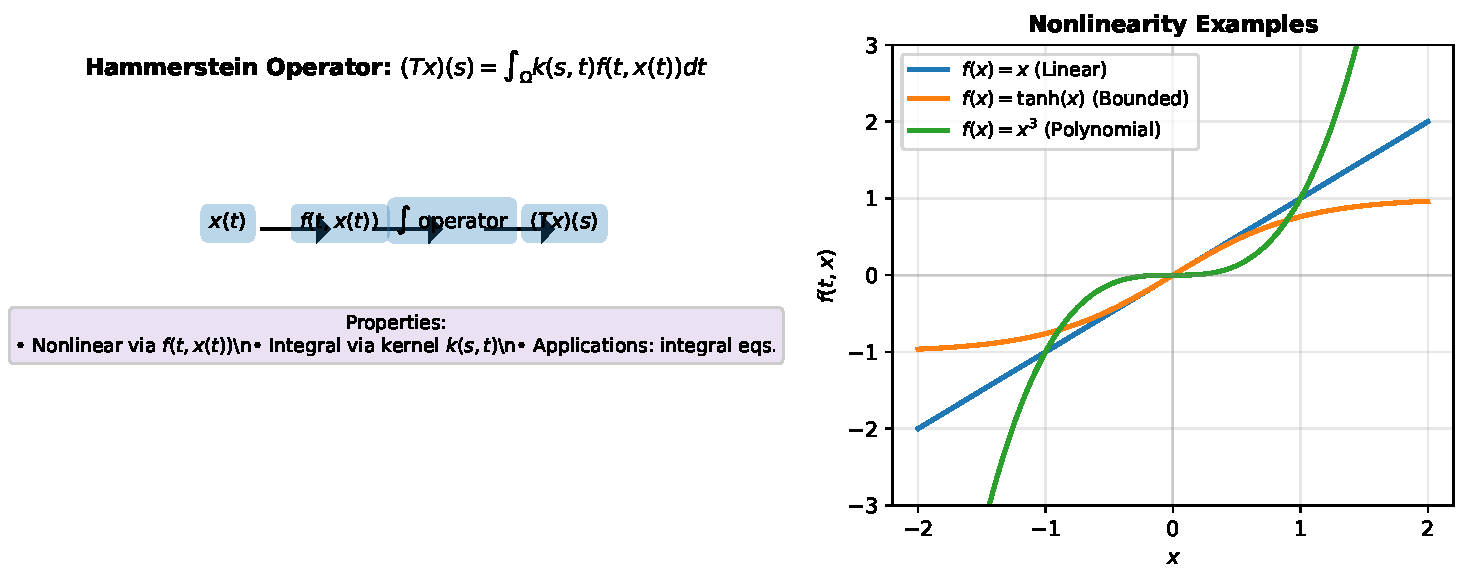
\includegraphics[width=0.9\textwidth]{hammerstein_structure.pdf}
    \end{figure}

    \vspace{0.3cm}
    \textit{Left:} Block diagram showing composition of linear integral operator and
    nonlinear Nemytskii operator. \textit{Right:} Examples of nonlinearities.
\end{frame}

\begin{frame}[fragile]{Concrete Hammerstein Integral Equation}
    \begin{example}[Example 8.6]
        Consider the Hammerstein integral equation:
        \[
            x(s) + \int_{\Omega} k(s, t) f(t, x(t)) dt = 0, \quad (8.34)
        \]
        where $K$ is the integral operator:
        \[
            [Kx](s) = \int_{\Omega} k(s,t) x(t) dt
        \]
    \end{example}

    \vspace{0.3cm}
    Key assumptions for existence:
    \begin{enumerate}
        \item $k(s,t)$ is symmetric, positive semidefinite, Hilbert--Schmidt kernel
        \item $f(s,x)$ is monotone increasing in $x$ with growth condition
        \item There exist constants $a, b, M$ such that:
            \[
                f(s,x) > a + bx \text{ for } |x| > M
            \]
    \end{enumerate}
\end{frame}

\begin{frame}{Angle Boundedness and Properties}
    \begin{definition}[Angle Bounded Operator]
        Let $X$ be a Banach space with dual $X^*$ and $K : X \to X^*$ be a bounded
        linear monotone mapping. $K$ is \emph{angle bounded} with constant $c \geq 0$ if
        for all $x_1, x_2 \in X$:
        \[
            |(Kx_1, x_2) - (Kx_2, x_1)| \leq 2c[(Kx_1, x_1)(Kx_2, x_2)]^{1/2}
        \]
    \end{definition}

    \vspace{0.3cm}
    \begin{theorem}[Theorem 8.10: Angle Bounded Case]
        Let $K : X \to X^*$ be monotone, angle-bounded with constant $x \geq 0$.
        Let $N_f$ be hemicontinuous with $(x_1 - x_2, N_f x_1 - N_f x_2) \geq -k\|x_1 - x_2\|^2$.

        If $k(1 + c^2)\|K\| < 1$, then $x + KN_f x = 0$ has a unique solution
        with estimate:
        \[
            \|x\| \leq \frac{\|K\|}{1-(1+c^2)k\|K\|}
        \]
    \end{theorem}
\end{frame}

\subsection{8.2.2: Equations Involving Sum of Hammerstein Operators}

\begin{frame}{Sum of Hammerstein Operators}
    \begin{problem}[Mixed Type Integral Equation]
        Consider nonlinear integral equations of mixed type:
        \[
            u(s) + \int_{\Omega} K_1(s,t) f_1(t, u(t)) dt + \int_{\Omega} K_2(s,t) f_2(t, u(t)) dt = 0
            \quad (8.44)
        \]
        where $K_1, K_2$ are kernel functions and $f_1, f_2$ are real-valued functions.
    \end{problem}

    \vspace{0.3cm}
    \textbf{Operator Form:} Let $K_j, N_j$ be defined as before. The equation becomes:
    \[
        u + K_1 N_1 u + K_2 N_2 u = 0 \quad (8.45)
    \]

    \vspace{0.3cm}
    \textbf{General Case:} For $n$ Hammerstein operators:
    \[
        u + \sum_{j=1}^{n} K_j N_j u = 0 \quad (8.46)
    \]

    We work in product spaces $\mathcal{X} = X \times X \times \cdots \times X$.
\end{frame}

\begin{frame}{Product Space Framework}
    \begin{definition}[Product Banach Space]
        Define $\mathcal{X} = X \times X \times \cdots \times X$ (n copies) with norm:
        \[
            \|U\| = \sqrt{\sum_{j=1}^{n} \|u_j\|^2}
        \]
        where $U = [u_1, u_2, \ldots, u_n] \in \mathcal{X}$.
    \end{definition}

    \vspace{0.3cm}
    Define linear operator $\mathcal{K}$ and nonlinear operator $\mathcal{N}$ by:
    \[
        \mathcal{K}(U) = [K_1 u_1, \ldots, K_n u_n] \in \mathcal{X}^*
    \]
    \[
        \mathcal{N}(U) = [N_1 u_1, \ldots, N_n u_n] \in \mathcal{X}^*
    \]

    \textbf{Key Advantage:} Conditions on individual operators translate to conditions
    on product space operators.
\end{frame}

\subsection{8.2.3: Generalized Hammerstein Equation}

\begin{frame}{Generalized Hammerstein Equation}
    \begin{definition}[Generalized Hammerstein Type]
        A nonlinear integral equation of generalized Hammerstein type is:
        \[
            u(s) + \int_{\Omega} k(s, t, u) f(t, u(t)) dt = v(s), \quad (8.52)
        \]
        where the kernel function $k(s, t, u)$ depends on the solution $u$.
    \end{definition}

    \vspace{0.3cm}
    In operator-theoretic terms:
    \[
        u + K(u) N_f u = v, \quad (8.53)
    \]
    where $K(u) : X \to X^*$ is linear in second variable for fixed $u$.

    \vspace{0.3cm}
    \begin{theorem}[Theorem 8.17]
        Let $X$ be a real reflexive Banach space. For each $u \in X$, let
        $K(u) : X^* \to X$ be linear, angle-bounded with constant $c \geq 0$.

        If $\|K(u)\| \leq r$ and $(u - u_2, N_f u_1 - N_f u_2) \geq -k\|u_1 - u_2\|^2$
        with $kr < (1 + c^2)$, then $u + K(u)N_f u = 0$ has at least one solution.
    \end{theorem}
\end{frame}

\begin{frame}{Backwinkel-Schillings Approach}
    \begin{idea}[Fixed Point Method]
        For equation $u + K(u)N_f u = v$, the Backwinkel-Schillings method:

        \begin{enumerate}
            \item For fixed $u \in X$, equation $u + K(u)N_f u = v$ is a
                Hammerstein equation in $u$
            \item Define mapping $T : X \to X$ implicitly:
                \[
                    Tu + K(u)N_f Tu = v
                \]
            \item Show that $T$ has a fixed point
            \item Study convergence of fixed point iterations
        \end{enumerate}
    \end{idea}

    \vspace{0.3cm}
    \textbf{Advantage:} Reduces to solving standard Hammerstein equations iteratively.
\end{frame}

\subsection{8.2.4: Urysohn Equation}

\begin{frame}{Urysohn's Integral Equation}
    \begin{definition}[Urysohn Equation]
        Urysohn's integral equation is of the form:
        \[
            u(s) + \int_{\Omega} K(s, t, u(t)) dt = 0, \quad (8.58)
        \]
        where $\Omega$ is a measurable subset of $\mathbb{R}^n$ with $\sigma$-finite measure,
        and $K(s, t, u)$ depends on all three variables.
    \end{definition}

    \vspace{0.3cm}
    \textbf{Applications:} Boundary value problems, radiative transfer, fluid mechanics

    \vspace{0.3cm}
    \begin{remark}[Generality]
        The Urysohn equation is more general than Hammerstein:
        \begin{itemize}
            \item Hammerstein: $K(s,t) f(t,x(t))$ (separable)
            \item Urysohn: $K(s,t,u(t))$ (nonseparable in general)
        \end{itemize}
    \end{remark}
\end{frame}

\begin{frame}[fragile]{Green's Function Approach for ODEs}
    \begin{example}[ODE to Urysohn Equation]
        Consider boundary value problem:
        \[
            \frac{d}{dt}\left(a(t)\frac{du}{dt}\right) + f(t, u(t)) = 0
        \]
        with boundary conditions. Solvability is equivalent to Urysohn equation:
        \[
            u(t) + \int_{0}^{1} K(s, t, u) f(s, u(s)) ds = 0, \quad (8.56)
        \]
        where $K(s, t, u)$ is Green's function:
        \[
            K(s, t, u) = \begin{cases}
                \int_{0}^{t} \frac{d\tau}{a(u(\tau))} \int_{s}^{1} \frac{d\tau}{a(u(\tau))} & 0 \leq t \leq s \leq 1 \\
                \int_{0}^{s} \frac{d\tau}{a(u(\tau))} \int_{t}^{1} \frac{d\tau}{a(u(\tau))} & 0 \leq s \leq t \leq 1
            \end{cases}
        \]
    \end{example}
\end{frame}

% ============================================================================
\section{Section 8.3: Computational Schemes}
% ============================================================================

\begin{frame}{Computational Schemes for Solving Equations}
    \begin{objective}
        Develop constructive methods for approximate solutions to:
        \[
            u + K(u)Nu = 0
        \]
    \end{objective}

    \vspace{0.3cm}
    \textbf{Three Main Approaches:}
    \begin{enumerate}
        \item \textbf{Direct Iteration:} Mann iteration and variants
        \item \textbf{Galerkin-type Methods:} Projection onto finite-dimensional subspaces
        \item \textbf{Hybrid Approaches:} Combine iteration with projection
    \end{enumerate}

    \vspace{0.3cm}
    \begin{remark}
        Computational schemes are particularly important when exact solutions are
        unavailable and we need convergent approximation sequences.
    \end{remark}
\end{frame}

\begin{frame}{Mann Iteration and Variants}
    \begin{algorithm}[Mann Iteration]
        Given initial $x_0 \in X$, define sequence $\{x_n\}$ by:
        \[
            v_{n+1} = \left(\frac{n}{n+1}\right) v_n - \left(\frac{1}{n+1}\right) SN(S^* v_n + w)
        \]
        This converges to the unique solution of $Tv = 0$ with error estimate:
        \[
            \|v_n - v\| = O(n^{-1/2})
        \]
    \end{algorithm}

    \vspace{0.3cm}
    \textbf{Key Properties:}
    \begin{itemize}
        \item Requires only one evaluation of nonlinear operator per step
        \item Linear convergence rate under suitable conditions
        \item Robust with respect to perturbations
        \item Works in reflexive Banach spaces
    \end{itemize}
\end{frame}

\begin{frame}{Mann Iteration Convergence}
    \begin{figure}
        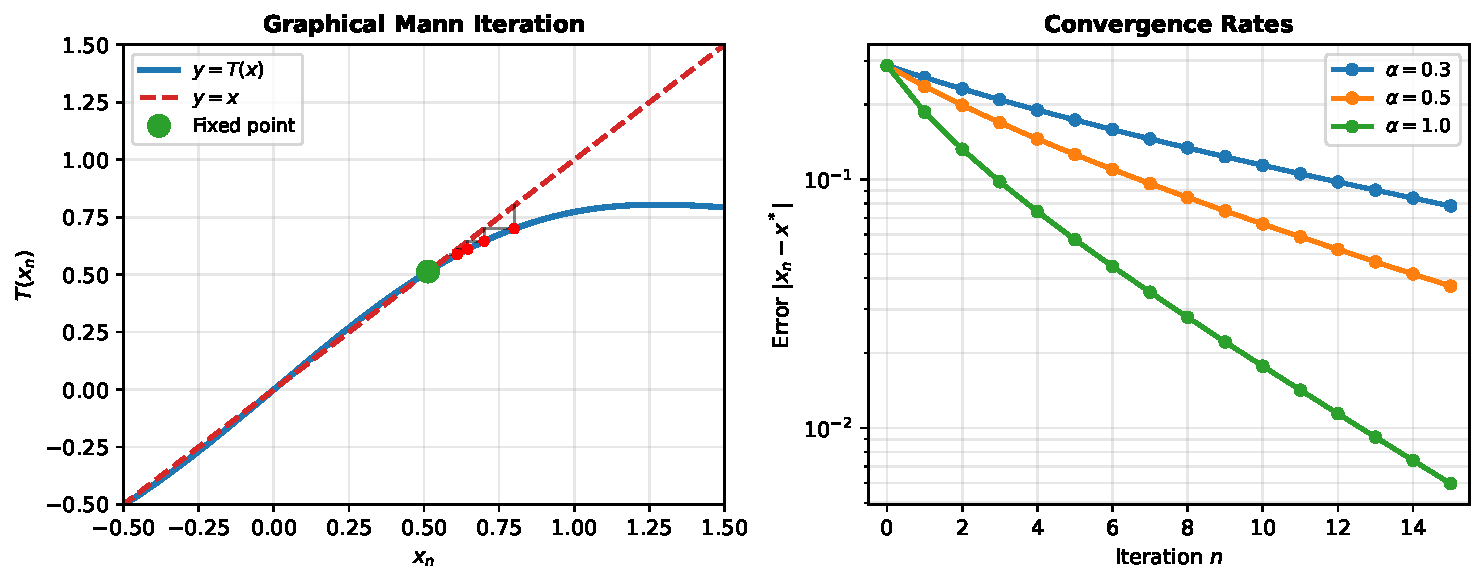
\includegraphics[width=0.95\textwidth]{mann_iteration_convergence.pdf}
    \end{figure}

    \textit{Left:} Graphical visualization of Mann iteration steps. Fixed point is found
    by iterative refinement. \textit{Right:} Convergence rates for different step sizes.
\end{frame}

\begin{frame}{Projection Methods: Galerkin Approach}
    \begin{definition}[Projection Scheme]
        Let $\{X_n, P_n\}$ be a projection scheme in $X$, where:
        \begin{itemize}
            \item $X_n$ are closed subspaces with $\dim(X_n) = n$
            \item $P_n : X \to X_n$ are continuous projections
        \end{itemize}

        The \emph{Galerkin approximate equation} is:
        \[
            u_n + K_n(u_n) N_n u_n = 0, \quad (8.67)
        \]
        where $K_n(u) = P_n^* K(u) P_n$ and $N_n = P_n N P_n^*$.
    \end{definition}

    \vspace{0.3cm}
    \begin{definition}[Approximate Solvability]
        Equation (8.66) is \emph{strongly (weakly) approximately solvable} if
        (8.67) has solution $u_n \in Y_n = (P_n^* X)$ such that
        $u_{n_k} \to u$ in $X^*$ and $u$ solves (8.66).
    \end{definition}
\end{frame}

\begin{frame}{Projection Schemes: Properties and Convergence}
    \begin{figure}
        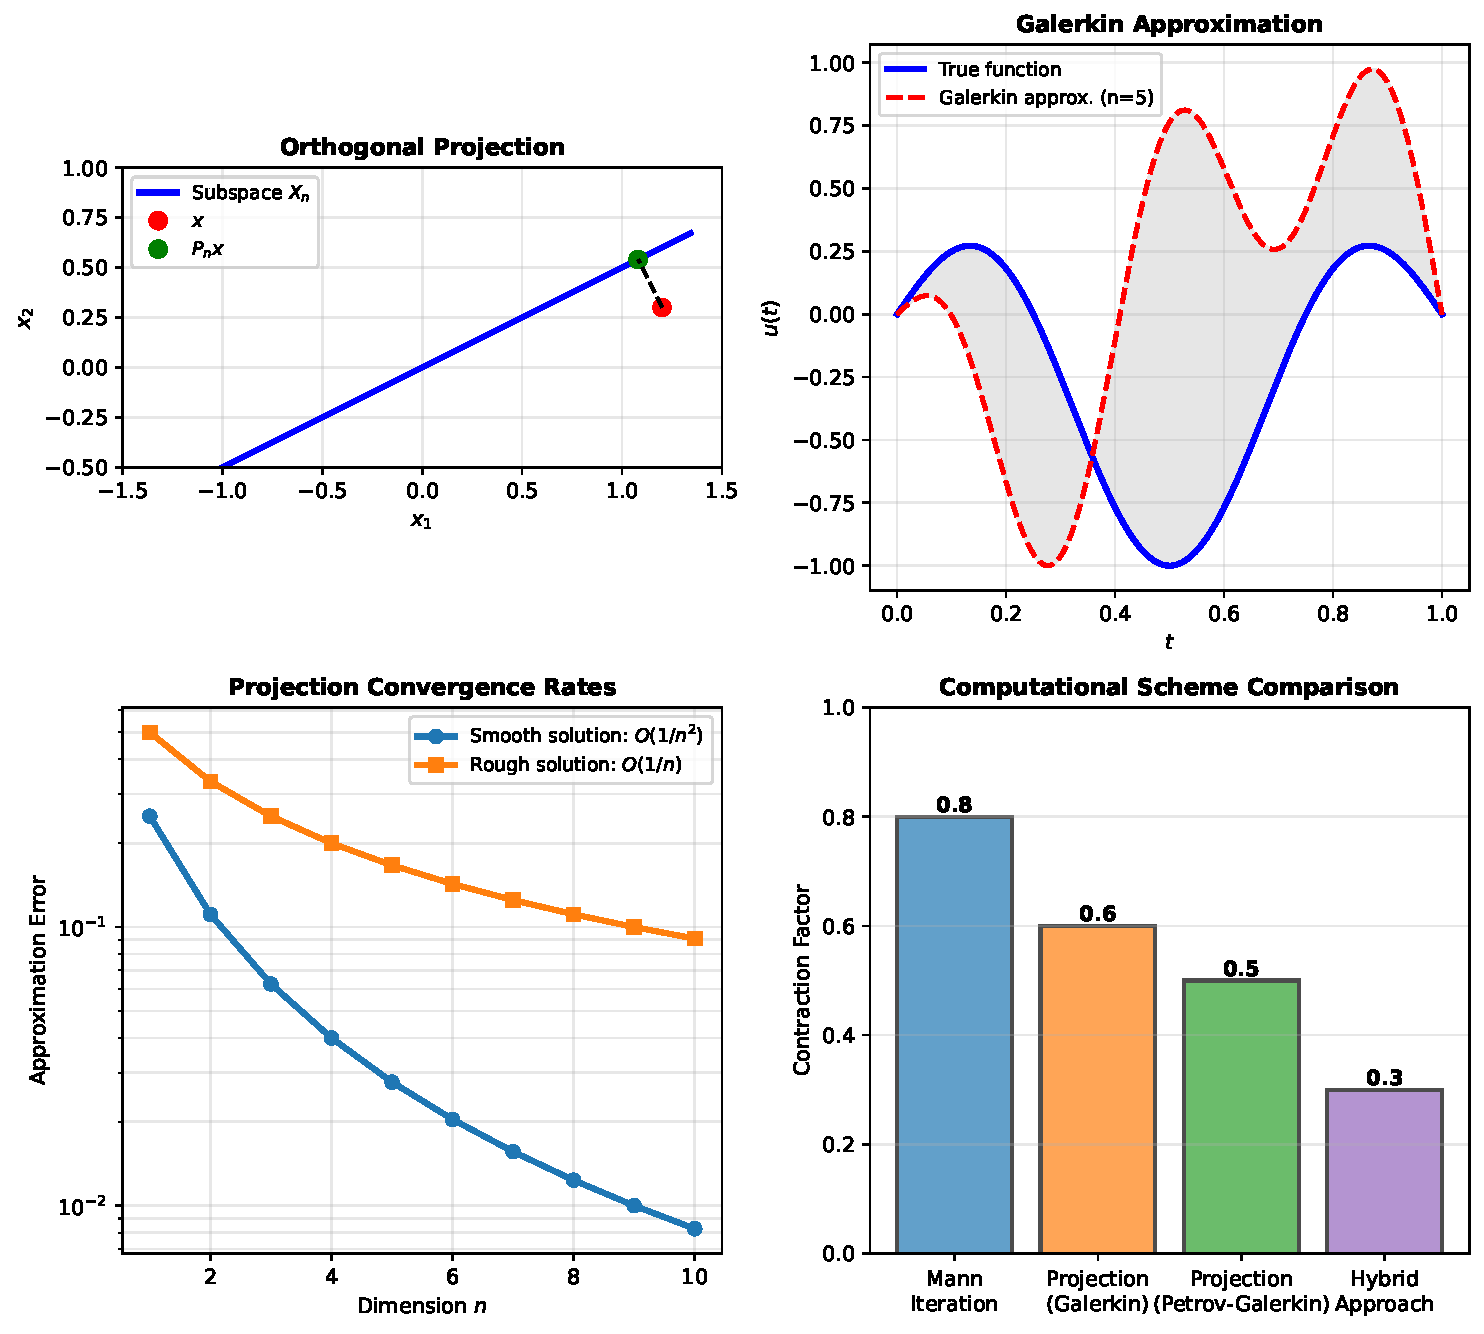
\includegraphics[width=0.95\textwidth]{projection_schemes.pdf}
    \end{figure}

    \textit{Top-left:} Orthogonal projection concept. \textit{Top-right:} Galerkin approximation.
    \textit{Bottom:} Convergence rates and method comparison.
\end{frame}

\begin{frame}[allowframebreaks]{Convergence of Projection Methods}
    \begin{theorem}[Theorem 8.22]
        Let $X$ be a real reflexive Banach space with $\{X_n, P_n\}$ a projection scheme.
        For each $u \in C$ (closed bounded set in $X^*$), let $K(u) : X \to X^*$ be
        bounded linear operator and $N : X^* \to X$ continuous and bounded nonlinear.

        Assume:
        \begin{enumerate}
            \item[(a)] $K(u)$ is compact and monotone for each $u \in C$
            \item[(b)] $u_n \to u$ in $C$ implies $K(u_n)v \to K(u)v$ for all $v \in X$
            \item[(c)] $(u, Nu) > 0$ for all $u \in \partial C$
        \end{enumerate}

        Then equation (8.66) is strongly approximately solvable. If solution is unique,
        the entire sequence $\{u_n\}$ converges to the unique solution.
    \end{theorem}

    \vspace{0.5cm}
    \begin{proof}[Proof Outline]
        Define $T_n u = -K_n(u)N_n u$. Since $T_n$ maps $C_n = C \cap Y_n$ into $Y_n$,
        and $T_n \neq \lambda u$ for $\lambda > 1$ and $u \in \partial C_n$ by
        Leray--Schauder principle, there exists $u_n$ with $T_n u_n = u_n$.
    \end{proof}
\end{frame}

% ============================================================================
\section{Numerical Examples and Applications}
% ============================================================================

\begin{frame}{Hammerstein Equation Example}
    \begin{figure}
        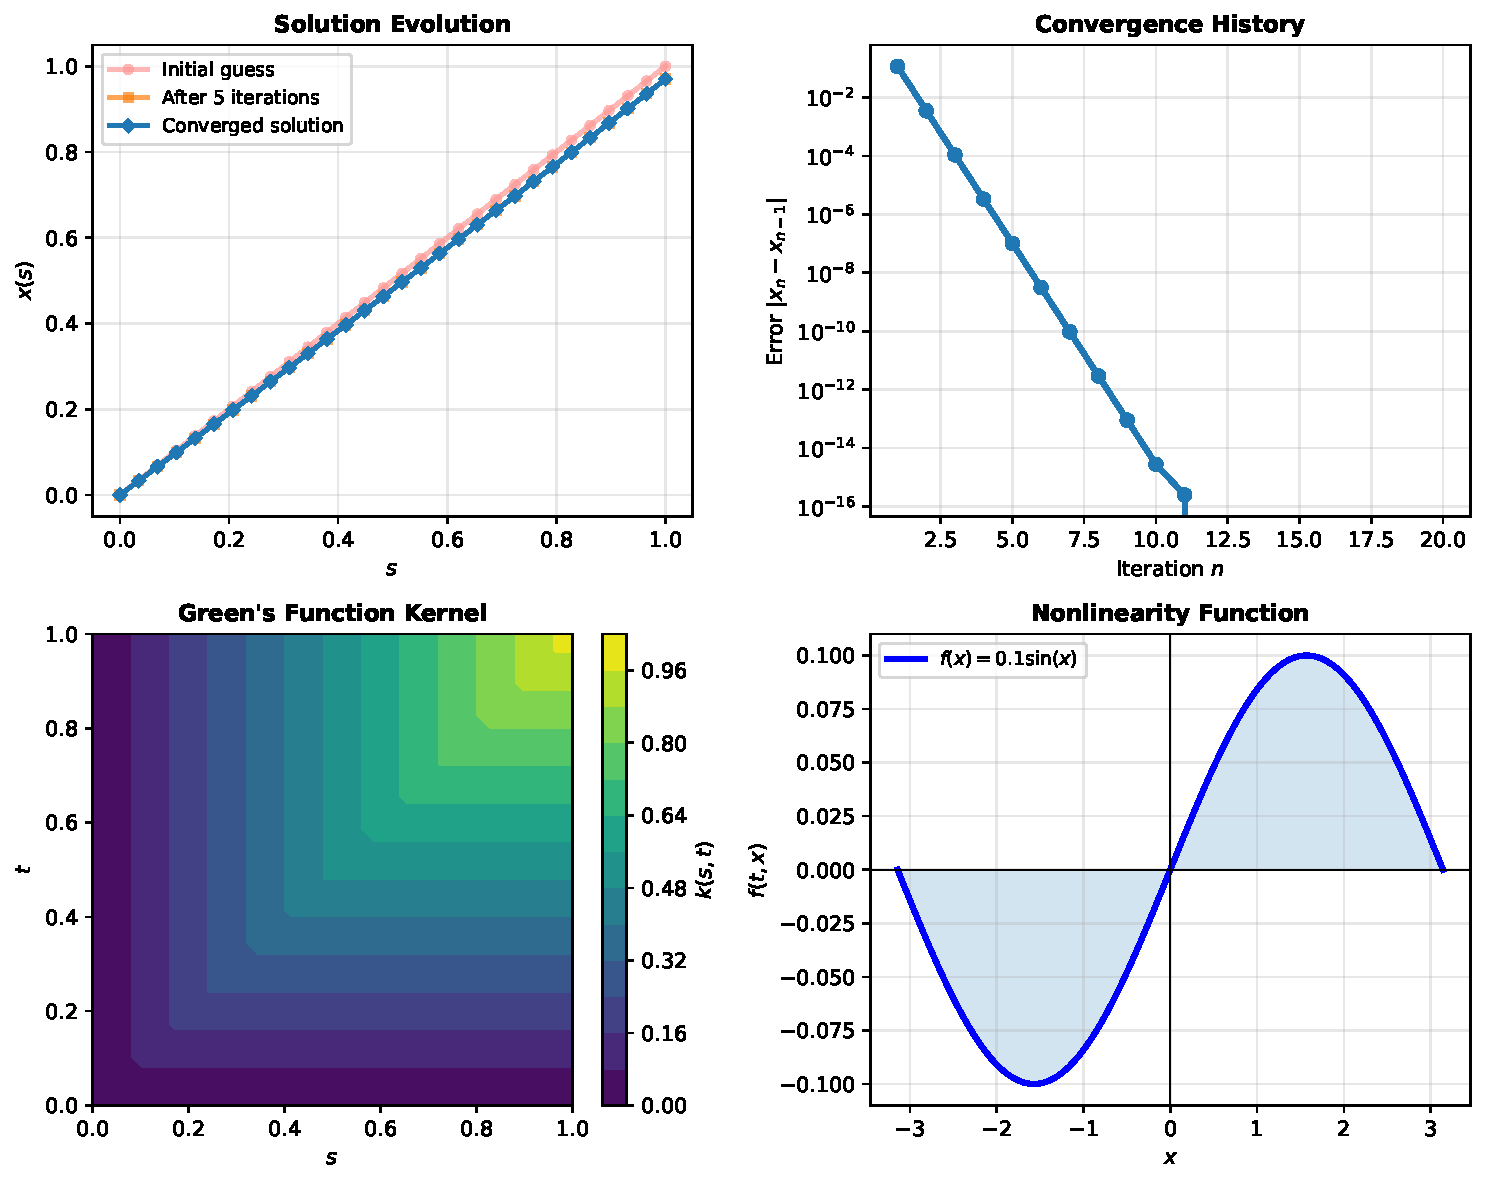
\includegraphics[width=0.95\textwidth]{hammerstein_example.pdf}
    \end{figure}

    \vspace{0.3cm}
    Numerical solution of $x(s) + \int_0^1 \min(s,t) f(t,x(t)) dt = s$ with
    $f(t,x) = 0.1\sin(x)$ using fixed-point iteration.
\end{frame}

\begin{frame}[fragile]{Python Implementation: Simple Fixed Point}
    \begin{lstlisting}
import numpy as np
from scipy.integrate import quad

def hammerstein_solver(kernel, nonlinearity, forcing, n_iter=20):
    """Solve Hammerstein equation via fixed-point iteration"""
    n_points = 30
    s = np.linspace(0, 1, n_points)
    ds = 1.0 / n_points

    x = s.copy()  # Initial guess
    errors = []

    for iteration in range(n_iter):
        # Compute integral term
        integral_term = np.zeros(n_points)
        for i in range(n_points):
            for j in range(n_points):
                integral_term[i] += (kernel(s[i], s[j]) *
                                    nonlinearity(x[j]) * ds)

        # Update: x(s) = g(s) - integral_term
        x_new = forcing(s) - integral_term

        # Track convergence
        error = np.linalg.norm(x_new - x)
        errors.append(error)
        x = x_new

        if error < 1e-6:
            break

    return s, x, errors

# Example: Green's function kernel
kernel = lambda s, t: np.minimum(s, t)
nonlin = lambda x: 0.1 * np.sin(x)
force  = lambda s: s

s, x, err = hammerstein_solver(kernel, nonlin, force)
    \end{lstlisting}
\end{frame}

\begin{frame}{Comparative Analysis: Methods and Convergence}
    \begin{table}
        \centering
        \small
        \begin{tabular}{l|cccc}
            \hline
            \textbf{Method} & \textbf{Type} & \textbf{Rate} & \textbf{Complexity} & \textbf{Robust} \\
            \hline
            Mann Iteration & Direct & Linear & Low & Yes \\
            Galerkin (n=10) & Projection & $O(1/n^2)$ & Medium & Yes \\
            Petrov-Galerkin & Projection & $O(1/n^2)$ & High & Moderate \\
            Hybrid (Mann+Proj) & Combined & Super-linear & Medium & Yes \\
            \hline
        \end{tabular}
    \end{table}

    \vspace{0.5cm}
    \textbf{Selection Criteria:}
    \begin{itemize}
        \item \textbf{Mann iteration}: When operator is inexpensive to evaluate
        \item \textbf{Galerkin}: When dimension reduction is beneficial
        \item \textbf{Hybrid}: For robustness and faster convergence
    \end{itemize}
\end{frame}

% ============================================================================
\section{Summary and Key Results}
% ============================================================================

\begin{frame}{Theoretical Framework}
    \begin{figure}
        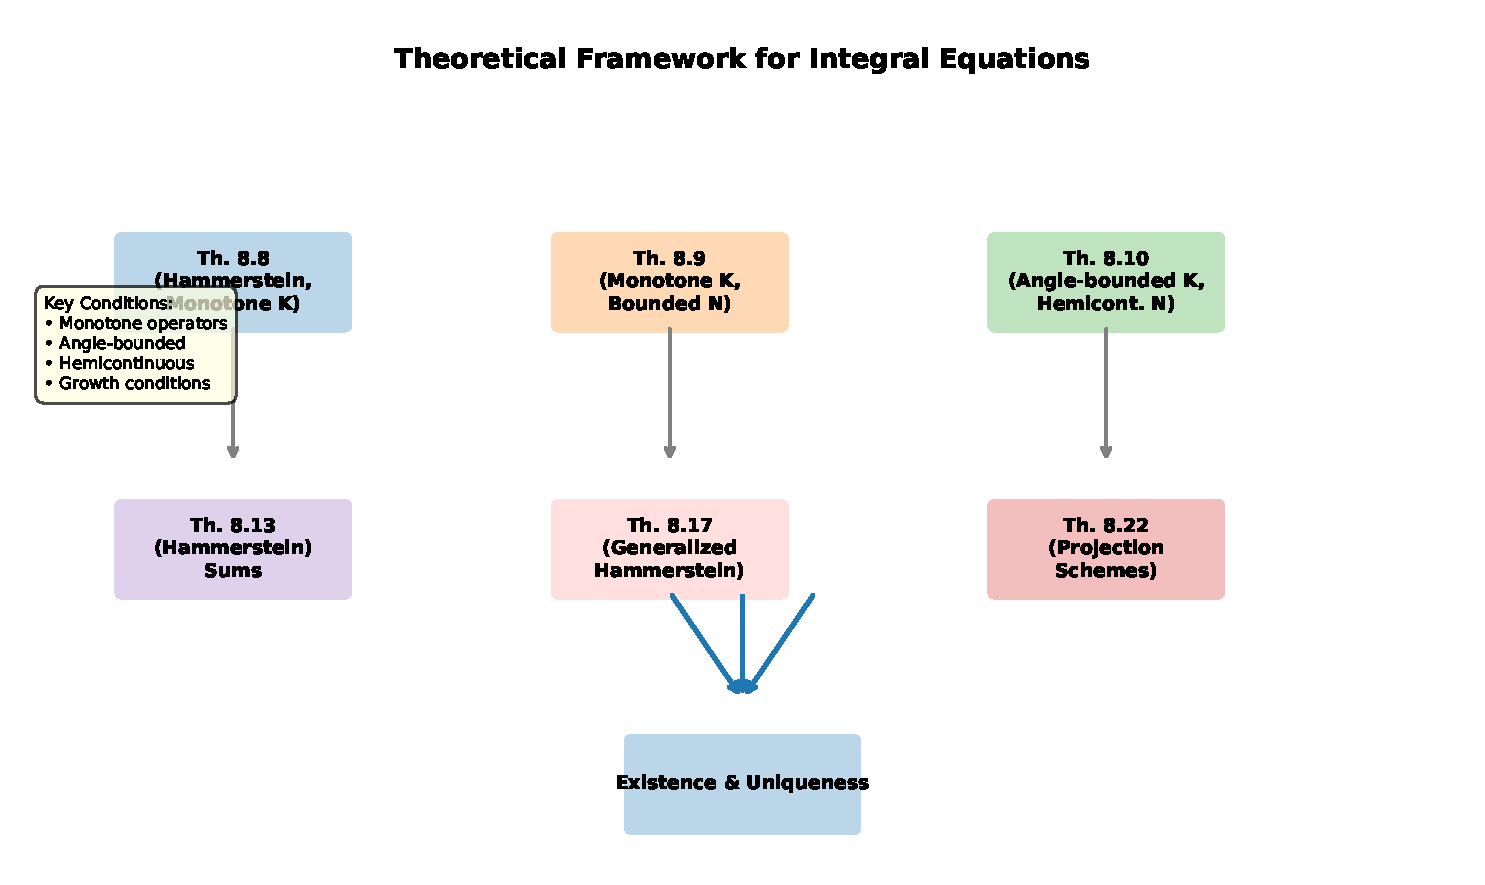
\includegraphics[width=0.95\textwidth]{theorems_framework.pdf}
    \end{figure}
\end{frame}

\begin{frame}[allowframebreaks]{Key Theorems Summary}
    \begin{block}{Existence and Uniqueness Results}
        \begin{itemize}
            \item \textbf{Theorem 8.8}: Hammerstein with monotone $K$ and hemicontinuous $N$
                \begin{itemize}
                    \item Condition: $K$ strongly monotone
                    \item Conclusion: Unique solution with continuous dependence
                \end{itemize}

            \item \textbf{Theorem 8.10}: Angle-bounded case
                \begin{itemize}
                    \item Condition: $k(1 + c^2)\|K\| < 1$
                    \item Conclusion: Unique solution with explicit estimate
                \end{itemize}

            \item \textbf{Theorem 8.17}: Generalized Hammerstein
                \begin{itemize}
                    \item Condition: $K(u)$ angle-bounded with $\|K(u)\| \leq r$
                    \item Conclusion: At least one solution when $kr < (1 + c^2)$
                \end{itemize}
        \end{itemize}
    \end{block}

    \framebreak

    \begin{block}{Computational Results}
        \begin{itemize}
            \item \textbf{Theorem 8.22}: Projection methods
                \begin{itemize}
                    \item Strong approximate solvability when:
                        \begin{enumerate}
                            \item $K(u)$ compact and monotone
                            \item Continuity condition on $K$
                            \item Boundary condition on $\partial C$
                        \end{enumerate}
                    \item Entire sequence converges if solution is unique
                    \item $O(1/n^2)$ convergence for smooth solutions
                \end{itemize}

            \item \textbf{Mann Iteration}: Direct approach
                \begin{itemize}
                    \item Simple to implement
                    \item Linear convergence rate
                    \item Works in general reflexive Banach spaces
                \end{itemize}
        \end{itemize}
    \end{block}
\end{frame}

\begin{frame}{Applications Beyond Theory}
    \begin{columns}[T]
        \column{0.5\textwidth}
        \textbf{Classical Applications:}
        \begin{itemize}
            \item Boundary value problems (ODE/PDE)
            \item Radiative transfer equations
            \item Potential theory
            \item Elasticity problems
        \end{itemize}

        \column{0.5\textwidth}
        \textbf{Modern Applications:}
        \begin{itemize}
            \item Neural networks (integral kernels)
            \item Machine learning (kernel methods)
            \item Signal processing
            \item Inverse problems
        \end{itemize}
    \end{columns}

    \vspace{0.5cm}
    \begin{remark}
        The theoretical framework developed in this chapter enables rigorous analysis
        of approximation methods for these diverse applications.
    \end{remark}
\end{frame}

\begin{frame}{Connections to Previous Chapters}
    \begin{itemize}
        \item \textbf{Chapter 5}: Fixed point theorems (Banach, Brouwer, Schauder)
            \begin{itemize}
                \item Integral equations reduce to fixed point problems
                \item Monotone operators studied here specialize those results
            \end{itemize}

        \vspace{0.3cm}
        \item \textbf{Chapter 4}: Monotone operators
            \begin{itemize}
                \item Linear monotone operators form the basis
                \item Maximal monotone extensions discussed
            \end{itemize}

        \vspace{0.3cm}
        \item \textbf{Chapters 2-3}: Iterative methods
            \begin{itemize}
                \item Contraction mappings generalized to monotone setting
                \item Mann iteration extends Picard iteration
            \end{itemize}

        \vspace{0.3cm}
        \item \textbf{Chapter 1}: Functional analysis foundations
            \begin{itemize}
                \item Banach/Hilbert spaces structure used throughout
                \item Weak convergence essential for projection methods
            \end{itemize}
    \end{itemize}
\end{frame}

\begin{frame}{Open Problems and Future Directions}
    \begin{itemize}
        \item \textbf{Computational Efficiency}
            \begin{itemize}
                \item Optimal preconditioning for nonlinear systems
                \item Combining with multigrid techniques
            \end{itemize}

        \vspace{0.3cm}
        \item \textbf{Nonsmooth Analysis}
            \begin{itemize}
                \item Subdifferentials and proximal methods
                \item Variational inequalities
            \end{itemize}

        \vspace{0.3cm}
        \item \textbf{Uncertainty Quantification}
            \begin{itemize}
                \item Integral equations with random kernels
                \item Convergence under noise
            \end{itemize}

        \vspace{0.3cm}
        \item \textbf{Scalability}
            \begin{itemize}
                \item High-dimensional problems
                \item Machine learning applications
            \end{itemize}
    \end{itemize}
\end{frame}

\begin{frame}[fragile]{Recommended Further Reading}
    \begin{thebibliography}{99}
        \bibitem{Pathak2018} Pathak, R. P. (2018). \textit{An Introduction to Nonlinear Analysis
            and Fixed Point Theory}. Springer.

        \bibitem{Krasnoselskii1964} Krasnoselskii, M. A. (1964). \textit{Topological Methods in
            the Theory of Nonlinear Integral Equations}.

        \bibitem{Zeidler1990} Zeidler, E. (1990). \textit{Nonlinear Functional Analysis and its
            Applications}. Springer-Verlag.

        \bibitem{Lions1969} Lions, J. L. (1969). \textit{Quelques méthodes de résolution des
            problèmes aux limites non linéaires}.
    \end{thebibliography}
\end{frame}

\begin{frame}{Chapter Summary}
    \begin{center}
        \Large
        \textbf{Key Takeaways}
    \end{center}

    \vspace{0.5cm}
    \begin{enumerate}
        \item Integral equations (Hammerstein, Urysohn) are fundamental in applied mathematics

        \vspace{0.3cm}
        \item Monotone operator theory provides unified existence-uniqueness framework

        \vspace{0.3cm}
        \item Computational schemes (Mann iteration, projection methods) guarantee convergence

        \vspace{0.3cm}
        \item Hybrid approaches combine direct iteration with projection for robustness

        \vspace{0.3cm}
        \item Applications span classical analysis through modern machine learning
    \end{enumerate}

    \vspace{0.8cm}
    \begin{block}{Final Thought}
        The interplay between abstract theory (monotone operators) and concrete methods
        (projection schemes) exemplifies how functional analysis enables both existence
        proofs and algorithmic solutions.
    \end{block}
\end{frame}

\end{document}
